\subsection{Weather:}
\label{sec:weather}
Since the early 1980's a major part of games have been there use of weather.
The weather used in games generally have one of two different uses.
The first use of weather in games is using the weather to affect gameplay such as Ouranos! (\citeyear{Ouranos80}) which uses it as the main game mechanic.
More recently Dear Ester (\citeyear{DearEsther12}) used the weather for the second reason which is as a way to add to the immersion the player feels when playing the game.
Figure \ref{fig:de_o} contains screenshots from both games and showcases how far the weather has come in games.
There are some games that utilise both types of weather in games, including Microsoft Flight Simulator X (\citeyear{MFS03}). 


\begin{figure}[ht!]
	\centering
	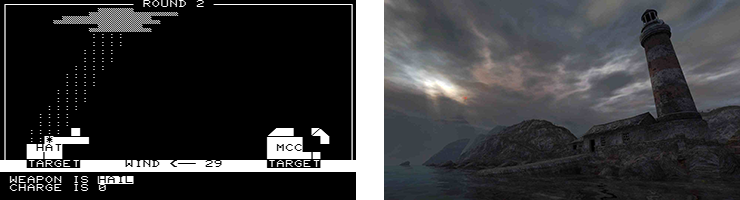
\includegraphics[width=\textwidth]{images/dear_esther.PNG}
	\caption{Left: Ouranos! (\citeyear{Ouranos80}), Right: Dear Ester (\citeyear{DearEsther12})}
	\label{fig:de_o}
\end{figure}


Looking closer at the types of weather used in games the use of clouds and rain stand out as the most recurring and notable aspects of weather as well as the most versatile examples of it use in games.
For example rain play different roles in two games Heavy Rain (\citeyear{HeavyRain10}) and rain (\citeyear{rain13}), but with it the games would not be as compelling as the currently are.
Figure \ref{fig:rain_heavy_rain} show screenshots from both games rain (\citeyear{rain13}) shows how rain is used to affect gameplay by allowing the player only to see the character in the rain, while Heavy Rain (\citeyear{HeavyRain10}) shows how the use of rain adds a depth that increase the film noir feel of the game.


\begin{figure}[ht!]
	\centering
	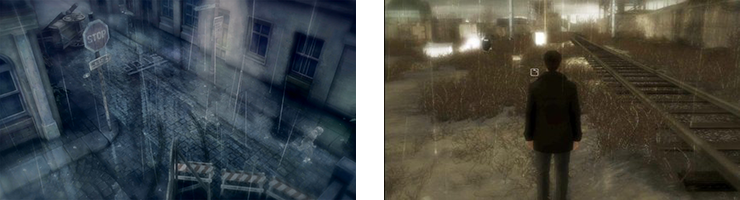
\includegraphics[width=\textwidth]{images/rain_heavy_rain.PNG}
	\caption{Left: rain (\citeyear{rain13}), Right: Heavy Rain (\citeyear{HeavyRain10})}
	\label{fig:rain_heavy_rain}
\end{figure}


When creating these games a number of different techniques were used to create and render the weather Ouranos! (\citeyear{Ouranos80}) uses ASCII because of the limitations at the time.
Games such as Super Mario Bros (\citeyear{SMB85}) use 2D sprites to render clouds on to the background and games like Tomb Raider (\citeyear{TombRaider13}) uses 3D scripted clouds.
2D games are also more likely to use 2D scrolling rain texture while 3D games are more likely to use a particle system to generate the rain.
Some games can use location data to simulate the correct weather at a given location such as NCAA Football 14 (\citeyear{NCAAF13}).
These games usually have a backup dynamic weather system which will be used if the game can't connect to the internet to collect data. 
Most games created use artistic representation of clouds instead of creating them in real time using equations.
Fluid dynamic equations can be used to represent the movement of any object made up of liquid or gas.
Basic clouds can be modelled by fluid dynamic equations, more advance clouds need extra equations for water continuity, thermodynamics, and buoyancy.
Using equations to generate the clouds will mean that the cloud will behave more like a real cloud than an artist's interpretation of a cloud.
When creating the cloud using these equations rain generation can be based proportionally on cloud size or by adding an extra equation to water continuity equations so rainfall is included.